% Author: Izaak Neutelings (September 2020)
% Inspiration: https://tex.stackexchange.com/questions/25531/adding-underbrace-in-tikz
\documentclass[border=3pt,tikz]{standalone}
\usepackage{tikz}
\usetikzlibrary{patterns,snakes}
\tikzstyle{ground}=[preaction={fill,top color=black!10,bottom color=black!5,shading angle=20},
                    fill,pattern=north east lines,draw=none,minimum width=0.3,minimum height=0.6]
\tikzstyle{mass}=[line width=0.6,red!30!black,fill=red!40!black!10,rounded corners=1,
                  top color=red!40!black!20,bottom color=red!40!black!10,shading angle=20]

\begin{document}


% HORIZONTAL floating
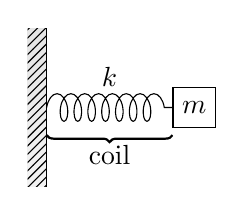
\begin{tikzpicture}
  \node (wall1) [ground, minimum height=2cm] {};
  \draw (wall1.north east) -- (wall1.south east);
  \node [draw,minimum width=0.5cm,minimum height=0.5cm] (mass) at (2,0) {$m$};
  \node (fix) at (0,0) {};
  \draw [ snake=coil, segment amplitude=5, segment length=5]
    (wall1.east) -- (mass)
    node [pos=0.5,above=4] {$k$};
  \draw [thick,decoration={brace,mirror,raise=10},decorate]
    (wall1.east) -- (mass)
    node [pos=0.5,below=10] {coil};
\end{tikzpicture}


\end{document}